\documentclass{article}

\usepackage{graphicx}
\usepackage{tikz}
\usepackage{tikzsymbols}
\usetikzlibrary{calc,patterns,shapes.geometric}
\pagestyle{empty}
\usepackage[margin=0pt]{geometry}
\geometry{papersize={14in,12in}}

\def\centerarc[#1](#2)(#3:#4:#5){\draw[#1] ($(#2)+({#5*cos(#3)},{#5*sin(#3)})$) arc (#3:#4:#5);}

\begin{document}
	\begin{figure}
		\centering
		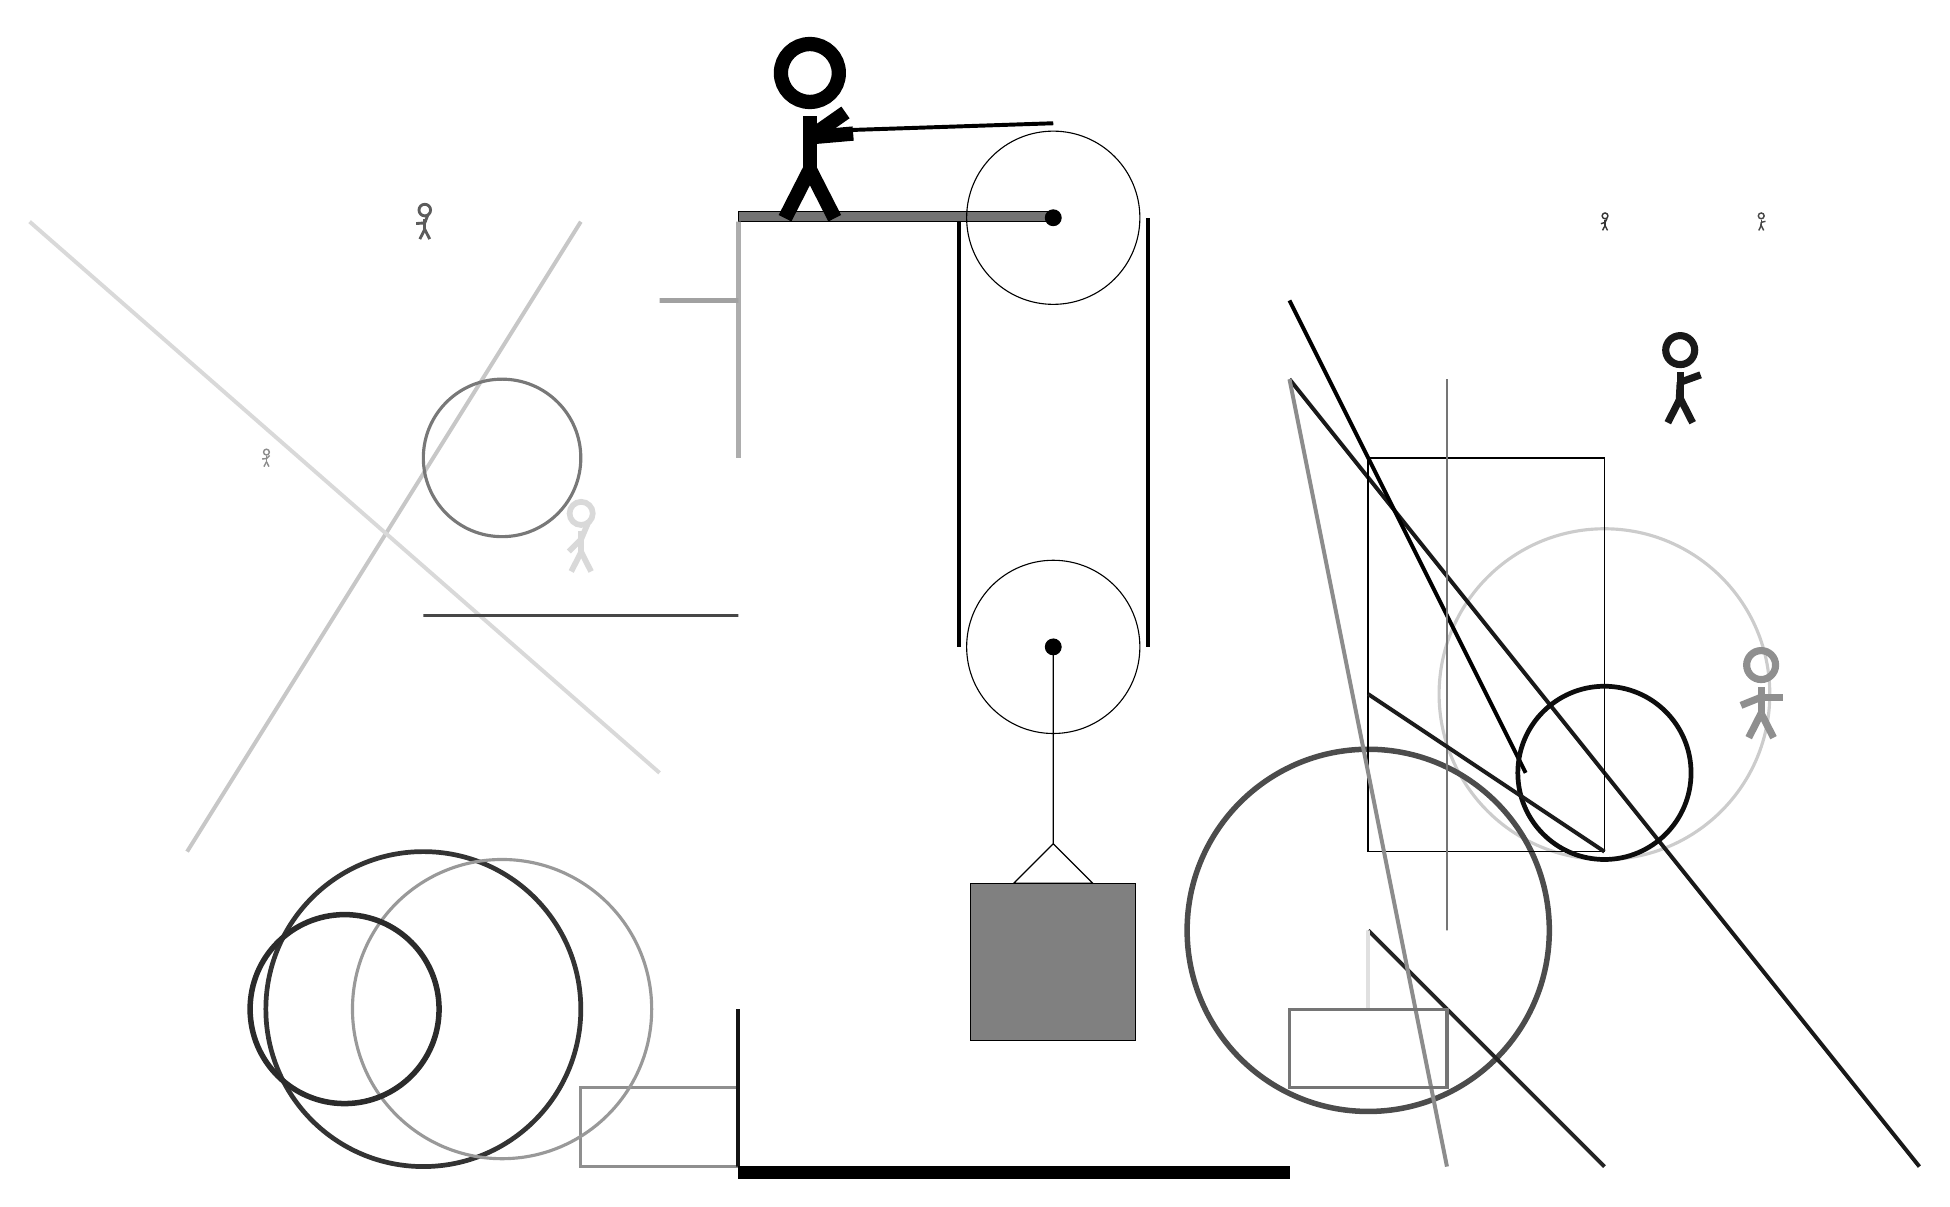
\begin{tikzpicture}
			%%%%% START %%%%%
			
			\draw[fill=black!55] (-2, 9) rectangle (2, 9.125);
			
			\draw (2, 3.6) circle (1.1);
			\draw[fill=black] (2, 3.6) circle (0.1);
			
			\draw (2, 9.05) circle (1.1);
			\draw[fill=black] (2, 9.05) circle (0.1);
			
			\draw (2, 3.6) -- (2, 1.1) -- (1.5, 0.6) -- (2.5, 0.6) -- (2, 1.1);
			\draw[fill=black!50] (0.95, 0.6) rectangle (3.05, -1.4);
			
			\draw[line width=0.5mm] (0.8, 9) -- (0.8, 3.6);
			\centerarc[line width=0.5mm](2, 3.6)(180:360:1.2000000000000002);
			\draw[line width=0.5mm](3.2, 3.6) -- (3.2, 9.05);
			\centerarc[line width=0.5mm](2, 9.05)(0:90:1.2000000000000002);
			\draw[line width=0.5mm](2, 10.25) -- (-1, 10.15);
			
			\draw [line width=0.4mm, color=black!20](9, 3) circle (2.1);
			
			\draw [line width=0.7mm, color=black!70](6, 0) circle (2.3);
			\draw[line width=0.6mm, color=black!32] (-2, 9) rectangle (-2, 6);
			\draw [line width=0.6mm, color=black!80](-6, -1) circle (2.0);
			
			\node[line width=0.2mm, color=black!79] at (9, 9) {\Strichmaxerl[1][19][63]};
			\draw[line width=0.5mm, color=black!90](5, 7) -- (13, -3);
			\draw[line width=0.5mm, color=black!22](-4, 9) -- (-9, 1);
			\draw[line width=0.7mm, color=black!37] (-3, 8) rectangle (-2, 8);
			\draw[line width=0.2mm, color=black!100] (6, 6) rectangle (9, 1);
			
			\draw [line width=0.4mm, color=black!53](-5, 6) circle (1.0);
			
			\node[line width=0.4mm, color=black!45] at (-8, 6) {\Strichmaxerl[1][6][44]};
			
			\node[line width=0.6mm, color=black!64] at (-6, 9) {\Strichmaxerl[2][4][69]};
			\draw[line width=0.4mm, color=black!44] (-4, -3) rectangle (-2, -2);
			
			\node[line width=0.6mm, color=black!44] at (11, 3) {\Strichmaxerl[5][22][0]};
			\node[line width=0.5mm, color=black!72] at (11, 9) {\Strichmaxerl[1][82][13]};
			\node[line width=0.2mm, color=black!15] at (-4, 5) {\Strichmaxerl[4][45][67]};
			
			\draw[line width=0.5mm, color=black!100](5, 8) -- (8, 2);
			
			\draw[line width=0.5mm, color=black!86](6, 0) -- (9, -3);
			\draw[line width=0.5mm, color=black!15](-3, 2) -- (-11, 9);
			\draw [line width=0.4mm, color=black!40](-5, -1) circle (1.9);
			\draw [line width=0.6mm, color=black!95](9, 2) circle (1.1);
			
			\draw[line width=0.2mm, color=black!54] (7, 0) rectangle (7, 7);
			
			\draw[line width=0.3mm, color=black!72] (-2, 4) rectangle (-6, 4);
			\draw[line width=0.5mm, color=black!45](5, 7) -- (7, -3);
			\draw [line width=0.7mm, color=black!83](-7, -1) circle (1.2);
			
			\draw[line width=0.5mm, color=black!89](6, 3) -- (9, 1);
			
			\draw[line width=0.5mm, color=black!12] (6, -1) rectangle (6, 0);
			\draw[line width=0.4mm, color=black!54] (7, -2) rectangle (5, -1);
			\draw[line width=0.5mm, color=black!92] (-2, -1) rectangle (-2, -3);
			
			\node[line width=0.6mm, color=black!90] at (10, 7) {\Strichmaxerl[5][87][20]};
			
			\node at (-1, 10.15) {\Strichmaxerl[10][-175][35]};
			
			\draw[fill=black] (-2, -3) rectangle (5, -3.15);
			
			%%%%% END %%%%%
		\end{tikzpicture}
	\end{figure}	
\end{document}